\documentclass{fkssolpub}

\usepackage[czech]{babel}
\usepackage{fontspec}
\usepackage{fkssugar}
\usepackage{amsmath}
\usepackage{graphicx}

\author{Ondřej Sedláček}
\school{Gymnázium Oty Pavla} 
\series{1p}
\problem{6} 

\begin{document}

\begin{figure}[h!]
	\begin{center}
		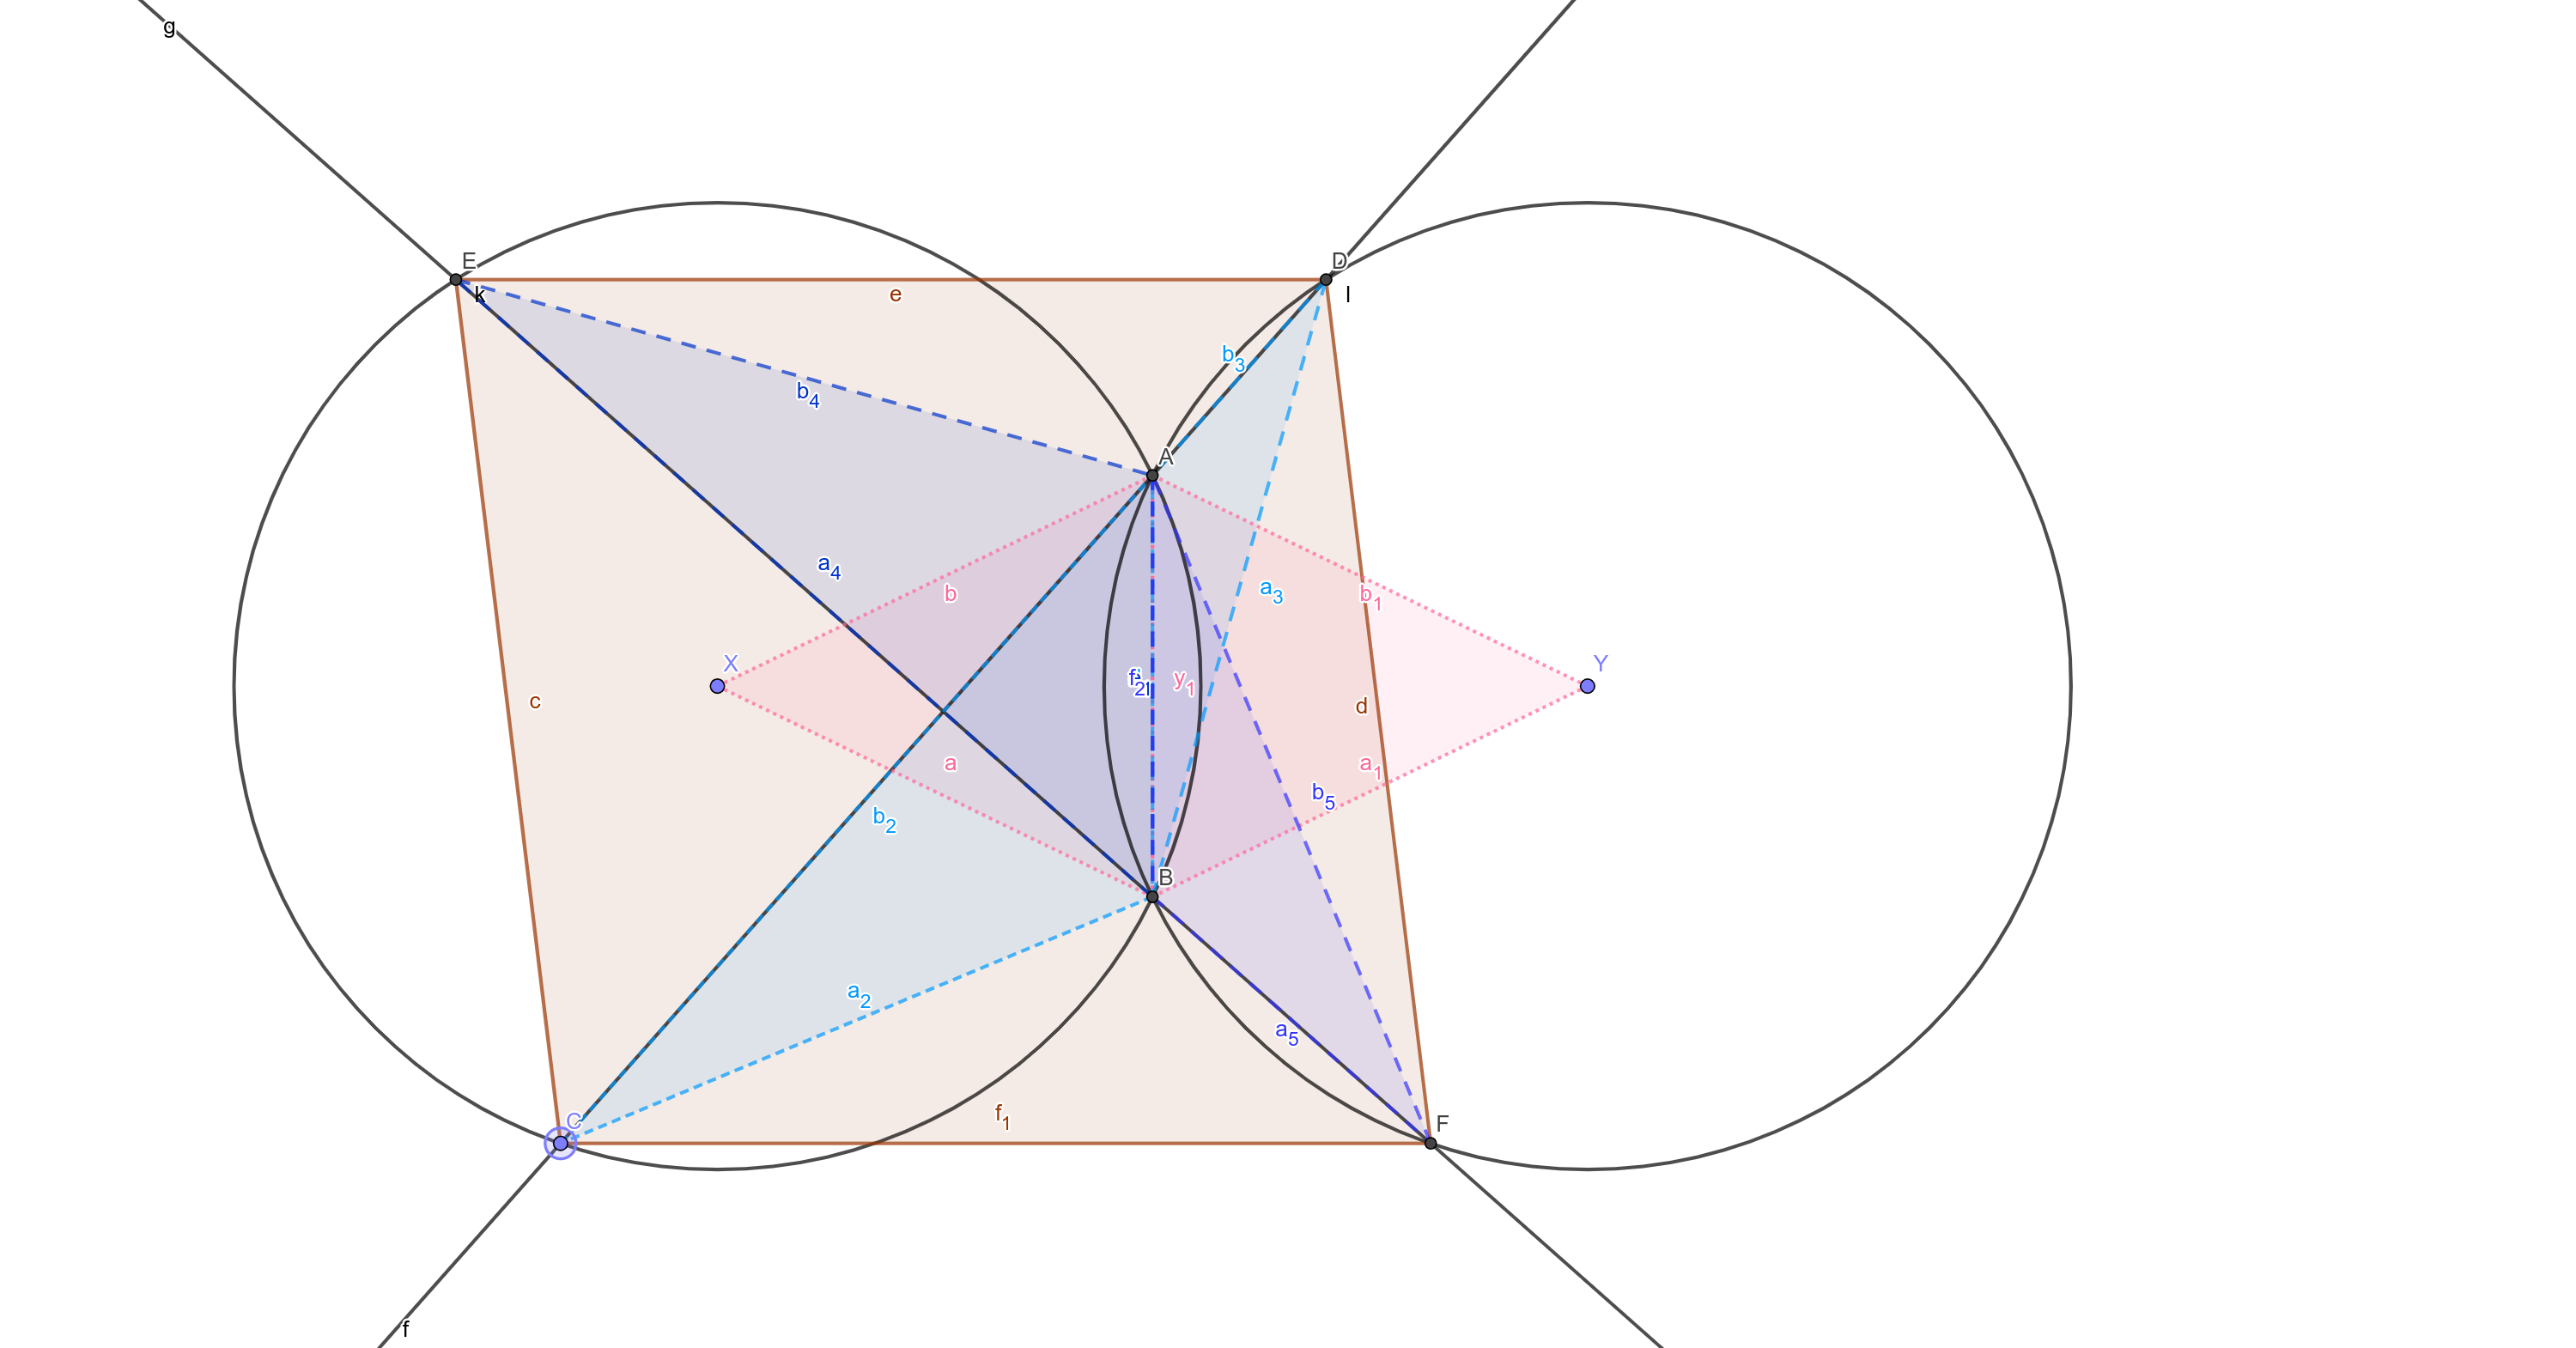
\includegraphics[width=0.95\textwidth]{6-fig-2.png}
	\end{center}
	\caption{Konstrukce, kdy žádný z bodů neleží na kratším oblouku $AB$}
	\label{fig:1}
\end{figure}

\begin{figure}[h!]
	\begin{center}
		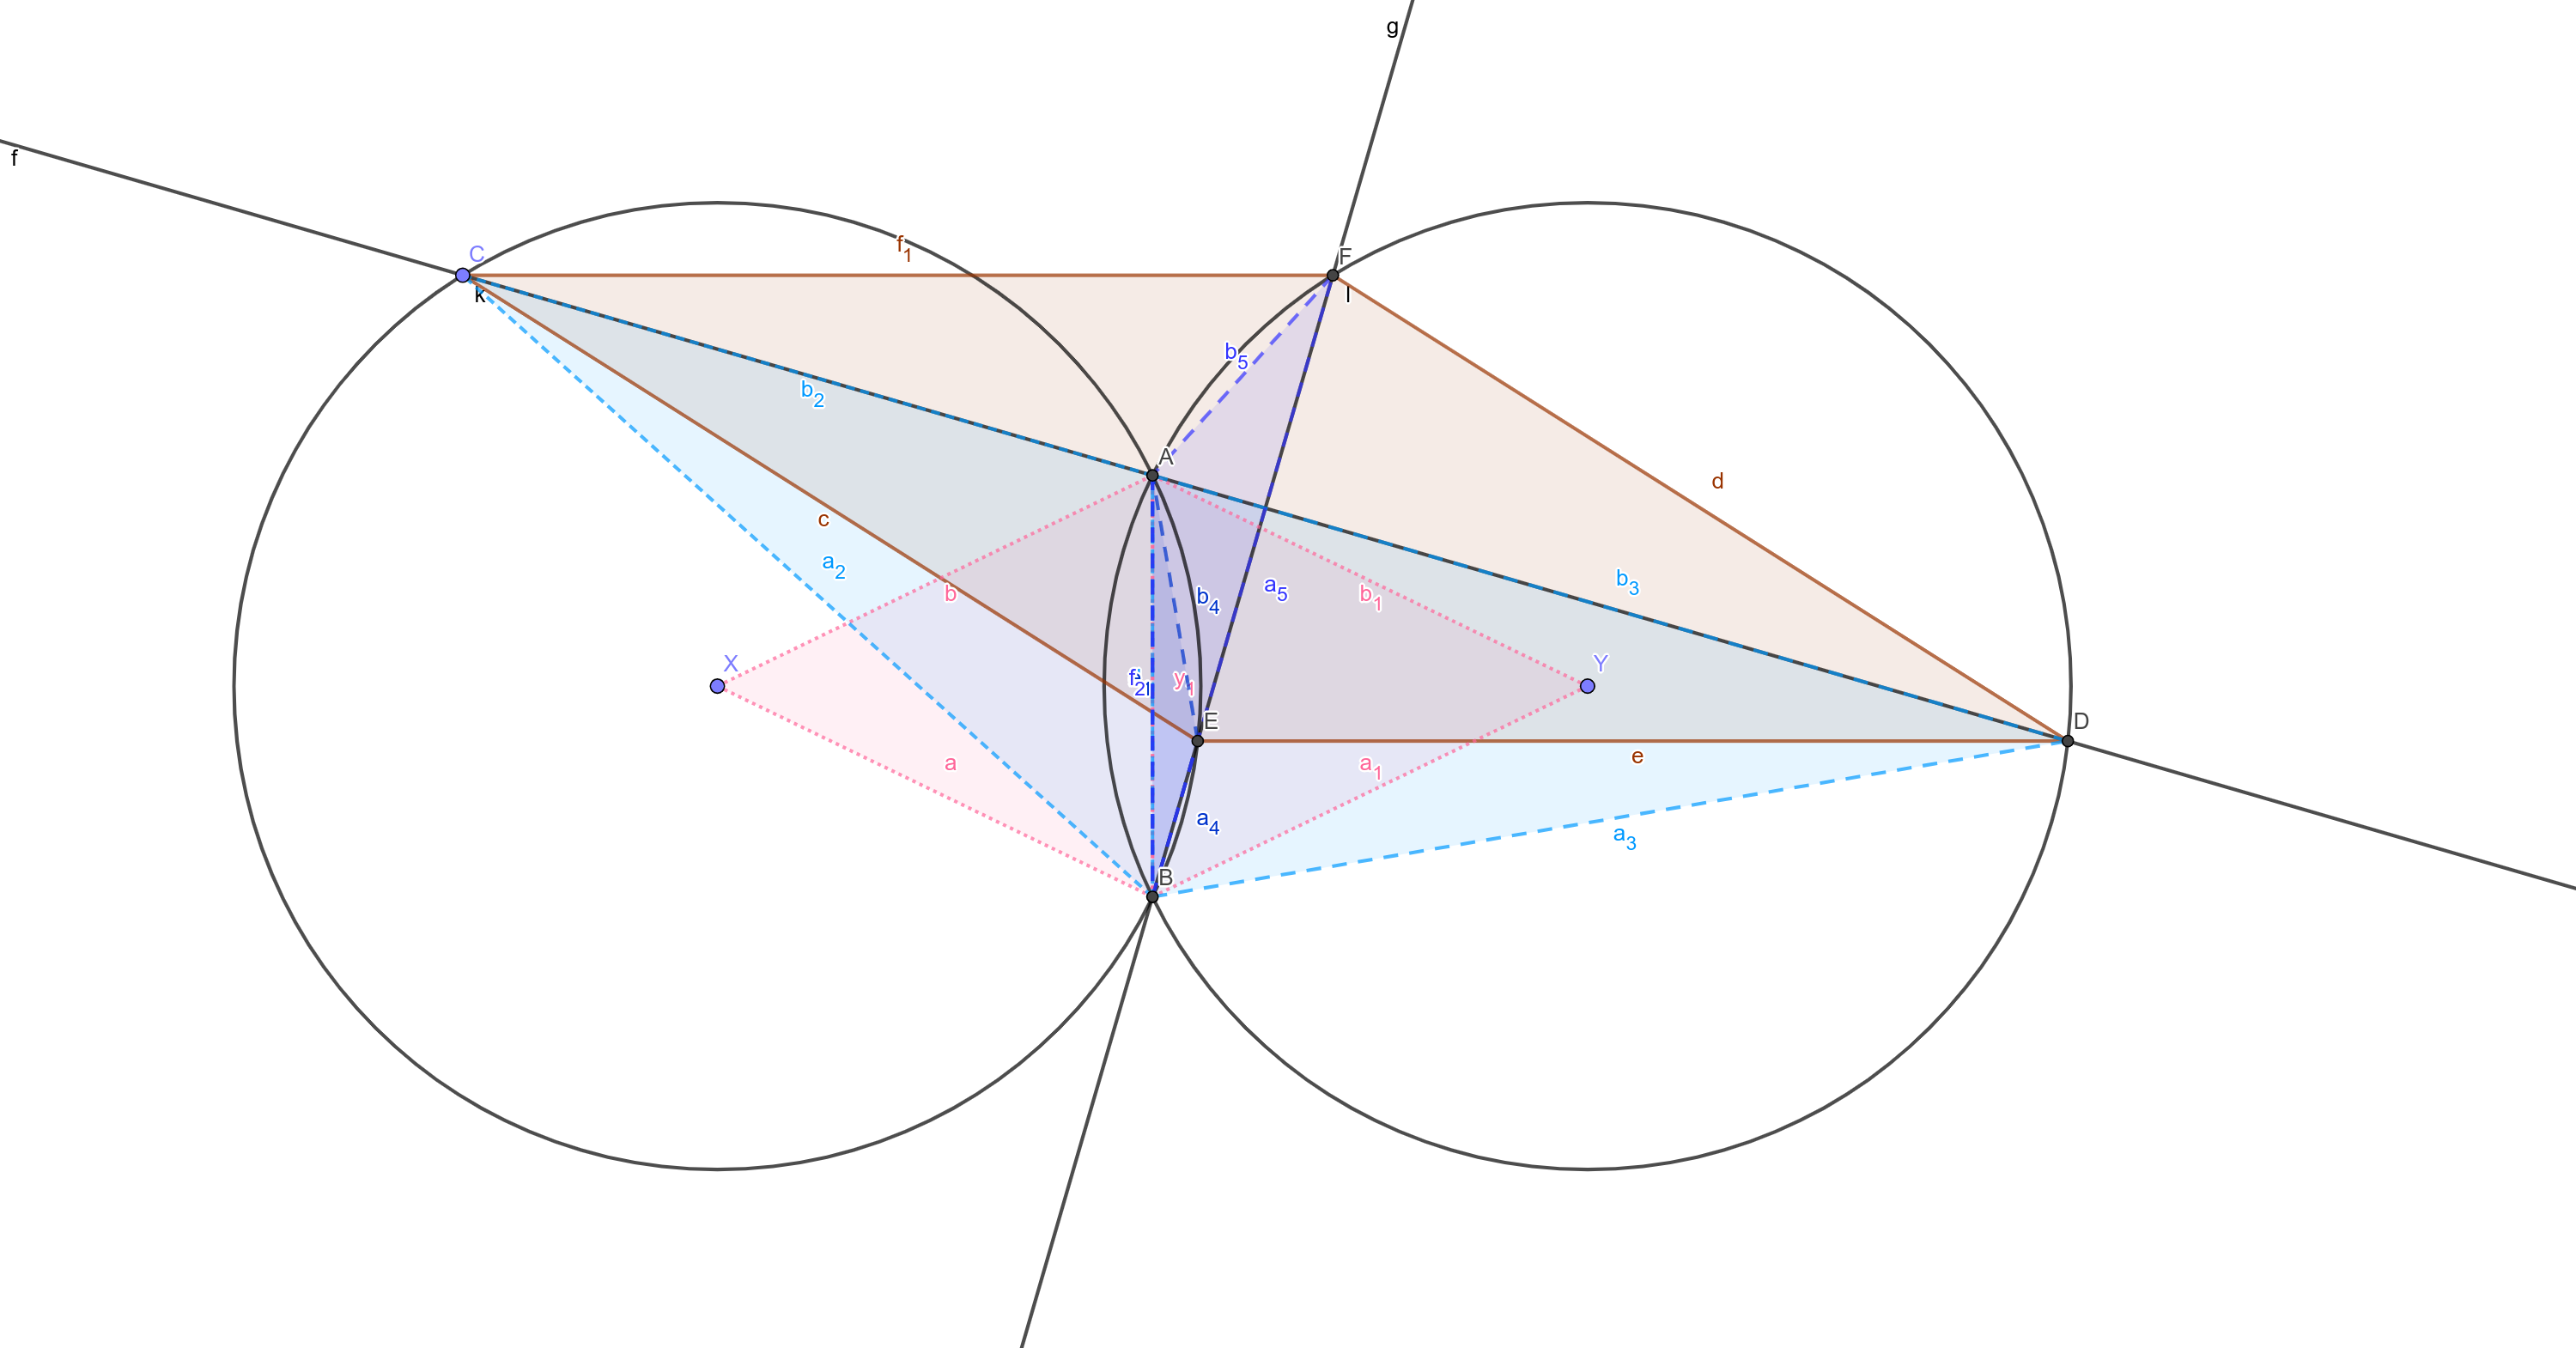
\includegraphics[width=0.95\textwidth]{6-fig-1.png}
	\end{center}
	\caption{Konstrukce, kdy bod $E$ leží na jednom z kratších oblouků $AB$}
	\label{fig:2}
\end{figure}

Je zřejmé, že podle věty sss jsou trojúhelníky $BAX$ a $ABY$ shodné, z čehož vyplývá, že $|\angle AXB| = |\angle BYA|$. A protože tyto úhly jsou středové, nad spojnicí $AB$ budou obvodové úhly u obou kružnic stejně velký.

Pokud dokážeme, že úhlopříčky $CD$ a $EF$ jsou osy daného čtyřúhelníku, dokážeme, že čtyřúhelníky $CEDF$ je kosočtverec, což je rovnoběžník. Abychom dokázali, že tyto úhlopříčky jsou osami, dokážeme, že trojúhelníky $DCB$ a $EFA$ jsou rovnoramenné se základnami $DC$ a $EF$. Toto snadno dokážeme pomocí obvodových úhlů.

Nejprve začneme s případem na obrázku \ref{fig:1}, kde je konstrukce, kdy žádný z bodů neleží na kratším oblouku $AB$. Tehdy protože středové úhly spojnice $AB$ k obou kružnicím jsou stejné, pak díky tomu platí, že $|\angle ACB| = |\angle BDA| = |\angle AEB| = |\angle BFA|$, čímž jsme dokázali, že tedy trojúhelníky $DCB$ a $EFA$ jsou rovnoramenné, jak jsme chtěli dokázat.

V případě na obrázku \ref{fig:2}, máme jeden z bodů na kratším oblouku $AB$, zde BÚNO bod $E$. Pro trojúhelník $DCB$ je dúkaz stejný jako v minulém případě, ale u druhého trojúhelníku není úhel $\angle BEA$ roven úhlu $\angle AEF$, ale jedná se o vnější úhel vůči tomuto úhlu. A protože obvodový úhel $\angle BEA$ se nachází na kratším oblouku, platí $|\angle BEA| = 180^{\circ} - |\angle BFA|$. Z toho je zřejmé, že $|\angle AEF| = |\angle BFA| = |\angle EFA|$, tím pádem jsme dokázali to samé jako v minulém případě.

A protože osy tohoto čtyřúhelníku prochází body $A$ a $B$, žádný jiný případ nastat nemůže (např. že by na kratším oblouku byly dva body čtyřúhelníku), čímž jsme dokázali tvrzení ze zadání. Q. E. D.


\end{document}
